\documentclass[preprint,12pt,3p,times]{elsarticle}
\biboptions{sort&compress}


%====package added by the authors
\usepackage[]{graphicx}
%\usepackage{float}
\usepackage{stackengine}
\usepackage{caption}
\usepackage{subfigure}
\usepackage{multirow}
\usepackage{amsmath,amssymb}
\usepackage{bm}
\usepackage{cases}
%\usepackage[round]{natbib}
\usepackage{booktabs}
\usepackage{soul,ulem}
\usepackage{setspace}
\usepackage[usenames, dvipsnames]{color}
\usepackage{lineno}
\usepackage{listings}
%\usepackage[nomarkers,tablesonly]{endfloat} % table managements
\usepackage[hidelinks]{hyperref} % for \url
\newcommand{\FS}[1]{{\textcolor{red}{\bf[FS: #1]}}}
\newcommand{\Mehdi}[1]{{\textcolor{OliveGreen}{\bf[Mehdi: #1]}}}
\newcommand{\rtwu}[1]{{\textcolor{blue}{\bf[#1]}}}
\newcommand{\rev}[1]{{\textcolor{blue}{#1}}}
%\renewcommand{\efloatseparator}{\vfill} % table managements
\soulregister\cite7
\soulregister\ref7
\soulregister\sout7
\soulregister\pageref7
\newcommand{\ed}[1]{{\textcolor{black}{#1}}}
\newcommand{\edit}[1]{{\textcolor{black}{#1}}}
\doublespacing
\DeclareRobustCommand{\hly}[1]{{\sethlcolor{yellow}\hl{#1}}}

% \journal{Computer Methods in Applied Mechanics and Engineering}
% \journal{Smart Materials and Structures}
% \journal{Mechanical Systems and Signal Processing}

\showboxdepth=\maxdimen
\showboxbreadth=\maxdimen

\begin{document}

\begin{frontmatter}

\title{Term Project: Deep Reinforcement Learning on Space Invaders}

\author[1]{Chia-Hung Chen}
\ead{r12543002@ntu.edu.tw}


\address[1]{Institute of Applied Mechanics, National Taiwan University, Taipei, Taiwan}

%=====================================


\begin{abstract}
This project delves into the use of reinforcement learning (RL) in Space Invaders, an arcade classic game.This project aims to create a player who can get the highest rewards in the game by use of sophisticated RL algorithms.Our major concern is on how RL techniques work such as Double Deep Q-Network (DDQ) that will enable the agent to successfully navigate through the game’s environment, make decisions strategically and garner maximum points.In this project, the details about the training process including any challenges faced plus our performance post-training, and successfully get high reward in the Space Invaders.
\newline
\end{abstract}

\begin{keyword}
Reinforcement Learning \sep Space Invaders \sep Double Deep Q-Networks
\end{keyword}

\end{frontmatter}

\section{Introduction}
Video games have long served as a enveriment for developing and testing reinforcement learning (RL) algorithms. Among the various genres, arcade games like Space Invaders present unique challenges due to their fast-paced, real-time nature and strategic complexity. RL, a subset of machine learning where agents learn to make decisions by network with their environment and receiving feedback.

Space Invaders, a game released in 1978\cite{GameSpy}, involves a player-controlled ship that must defend against waves of descending aliens by shooting them down while avoiding their attacks. The game's simplicity in rules but complexity in strategy makes it an ideal candidate for RL research. In this project, we leverage RL techniques to develop a agent that can autonomously play Space Invaders, aiming to achieve high scores or rewards by learning optimal strategies through trial and error.

The primary objective is to implement and evaluate RL algorithm, such as Double Deep Q-Network (DDQ)\cite{van2016deep}, to understand their effectiveness in this gaming context. We will discuss the training process, including the setup of the environment, reward structure, and the computational loss.

Through this project, we aim to contribute to the growing body of research on applying RL to video games, providing insights into the capabilities and limitations of current RL methodologies. The findings could have broader implications for the application of RL in other real-time, interactive systems beyond gaming.

\section{Literature Review}

Deep reinforcement learning (DRL) has become a significant focus within artificial intelligence research, particularly in its application to video games. This literature review synthesizes findings from various studies to provide an overview of the progress and challenges in this field.

\subsection{General Overview of DRL}
Deep reinforcement learning combines reinforcement learning (RL) with deep learning (DL), allowing agents to learn optimal behaviors through trial and error using neural networks to approximate the value functions or policies. This approach has been particularly successful in complex environments, such as video games, where traditional RL methods struggle with high-dimensional state spaces\cite{li2017deep}.

The seminal work by Mnih et al. (2015) demonstrated the potential of DRL by achieving human-level performance on several Atari 2600 games using a deep Q-network (DQN)\cite{mnih2015human}. This study used a convolutional neural network to approximate the Q -value function, enabling the agent to learn from raw pixel inputs, a significant advancement over previous methods that relied on hand-crafted features.

\subsection{Advances in DRL Algorithms}
Subsequent research has focused on improving the stability and performance of DRL algorithms. One notable improvement is the introduction of the double Q-learning algorithm, which addresses the overestimation bias in standard Q-learning by decoupling the action selection from the Q-value estimation\cite{van2016deep}. This technique significantly enhances the stability and performance of DRL agents.

Another critical development is the dueling network architecture proposed by Wang et al., which separates the representation of state values and advantage functions within the network. This architecture improves the efficiency of learning by allowing the network to generalize learning across actions without significant changes to the underlying RL algorithm\cite{wang2016dueling}.

\subsection{Application in Video Games}
The application of DRL in video games has extended beyond Atari games to more complex environments. The General Video Game AI (GVGAI) framework, as described by Torrado et al. (2018), provides a benchmark for testing the generalization capabilities of DRL algorithms across various games\cite{torrado2018deep}. This framework allows researchers to assess how well DRL agents can adapt to new and unseen games, which is crucial for developing more versatile AI.

In addition to general frameworks, specific studies have focused on improving decision-making efficiency in video games. Ji and Xiao (2020) proposed an improved deep Q-learning algorithm with priority experience replay to enhance the agent's learning efficiency by selectively replaying more informative experiences\cite{ji2020improving}. This method has shown to improve the performance of agents in image-based games by optimizing the learning process.

\subsection{Challenges and Variability}
Despite these advancements, DRL faces significant challenges, particularly in the reproducibility and variability of results. Clary et al. (2019) highlighted the issue of variability in DRL agents' performance due to the stochastic nature of training processes and the environment\cite{clary2019let}. argue that evaluating DRL agents based on single-point estimates can be misleading and advocate for reporting performance distributions to better capture the variability and reliability of the results.

\section{Method}

The goal of this project is to develop and evaluate a reinforcement learning (RL) agent capable of playing the classic arcade game Space Invaders. The agent will be trained using Double Deep Q-Network (DDQ), a popular RL algorithm that combines Q-learning with deep neural networks to handle high-dimensional sensory inputs. The following sections outline the environment setup, the architecture of the RL agent, the training process, and the evaluation metrics used to assess the agent's performance.

\subsection{Environment Setup}
\textbf{Game Environment}: Space Invaders is a classic arcade game where the player controls a ship at the bottom of the screen, tasked with shooting descending aliens while avoiding their attacks. The game environment is simulated using the OpenAI Gym, which provides an interface for interacting with the game and obtaining observations and rewards.

\textbf{State Representation}: The state or environment of the game is represented by raw pixel data from the game screen. Each state is an (210, 160, 3) image with four stacks, capturing the most recent four frames to provide a sense of motion to the agent. Then for easy training the image would compress to (84, 64, 1) gray scale image. The state is as following Fig.\ref{figlabel1}.

\begin{figure}[!t]
\centering
\subfigure[]{{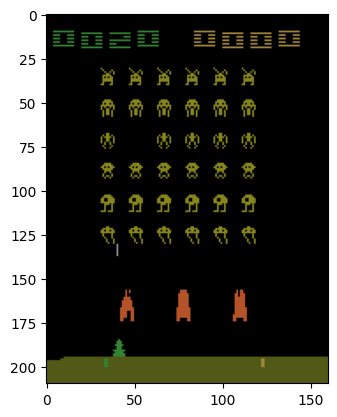
\includegraphics[width=.4\textwidth]{space_invaders1.png}}\label{f_scatterer_a}}
\subfigure[]{{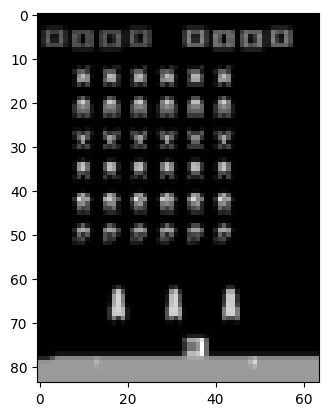
\includegraphics[width=.4\textwidth]{space_invaders2.png}}\label{f_scatterer_b}}
\caption{\label{figlabel1} The state or environment: (a) Original state with RGB color (b) The state with only gray scalier after prepossessing.}
\end{figure}

\textbf{Action Space}: The action space consists of six discrete actions corresponding to the possible moves in the game: move left, move right, fire, move left and fire, move right and fire, and no-op (do nothing).

\textbf{Reward Structure}: The agent receives a positive reward for hitting an alien and a negative reward for losing a life. The primary objective is to maximize the cumulative score over multiple episodes of gameplay.

\subsection{Architecture of the RL Agent}
\textbf{Double Deep Q-Network (DDQ)}: The DDQ architecture consists of two convolutional neural network (CNN) designed to process the raw pixel inputs, output \(Q_{online}\) and \(Q_{target}\) and for each action. The network architecture is as follows:

\begin{table}[!h]
\centering
\caption{\label{t_data_stats}The DDQ architecture of Space Invader}
\begin{tabular}{p{4.5cm} p{2.5cm} p{2.5cm} p{2.5cm} p{2.5cm}}
\hline
Layers                 & In Channels & Out Channels & Kernel Size & Stride \\ \hline
Convolutional Layer    & 4           & 32           & 8           & 4 \\
ReLU                   & -           & -            & -           & - \\
Convolutional Layer    & 32          & 64           & 4           & 2 \\
ReLU                   & -           & -            & -           & - \\
Convolutional Layer    & 64          & 64           & 3           & 1 \\
ReLU                   & -           & -            & -           & - \\
Flatten                & -           & -            & -           & - \\
Linear                 & 1792        & 512          & -           & - \\
ReLU                   & -           & -            & -           & - \\
Linear                 & 512         & 6            & -           & - \\ \hline
\end{tabular}
\end{table}

Therefore, The \(Q_{online}\) and \(Q_{target}\) would share feature, but separate the Fully-Connection Layer. The weighst of \(\theta_{target}\) (the parameters of \(Q_{target}\)) would be frozen and \(\theta_{online}\) would not. The setting is as following:

\begin{lstlisting}[language=Python]
# Q_target parameters are frozen.
for p in self.target.parameters():
    p.requires_grad = False
\end{lstlisting}

\subsection{Training Process}
\textbf{Experience Recall}: The agent uses an experience recall buffer to store transitions (state, action, reward, next state). During training, random minibatches of transitions are sampled from this buffer to break the correlation between consecutive experiences and stabilize training. The recall function shows below:

\begin{lstlisting}[language=Python]
def recall(self):
    batch = self.memory.sample(self.batch_size).to(self.device)
    state, next_state, action, reward, done = (batch.get(key) for key in ("state", "next_state", "action", "reward", "done"))
    return state, next_state, action.squeeze(), reward.squeeze(), done.squeeze()
\end{lstlisting}

\textbf{Exploration Decay Policy}: The agent follows an exploration decay policy to balance exploration and exploitation. The exploration rate value starts high to encourage exploration and gradually decreases to favor exploitation as training progresses. The exploration decay calculation shows below:

\begin{lstlisting}[language=Python]
# decrease exploration_rate
self.exploration_rate *= self.exploration_rate_decay
self.exploration_rate = max(self.exploration_rate_min, self.exploration_rate)
\end{lstlisting}

\textbf{TD Estimate and TD Target}: TD Estimate is the predicted optimal \(Q^{*}\) for a given state \(s\)
\begin{equation*}\label{eq_kernel}
    TD_{e}=Q^{*}_{online}(s,a)
\end{equation*}
, and TD Target is aggregation of current reward and the estimated \(Q^{*}\) in the next state \(s'\).
\begin{equation*}\label{eq_kernel}
    a'=argmax_{a}Q_{online}(s', a)
\end{equation*}
\begin{equation*}\label{eq_kernel}
    TD_{t}=r + \gamma Q^{*}_{target}(s',a')
\end{equation*}

\textbf{Optimization}: The DDQ is trained using the Adam optimizer. The loss function is the Smooth L1 Loss between the \(TD_{e}\) and the \(TD_{t}\) for updating \(\theta_{online}\)
\begin{equation*}\label{eq_kernel}
    \theta _{omline} \leftarrow \theta _{omline} + \alpha \bigtriangledown (TD_{e}-TD_{t})
\end{equation*}
, and the \(\theta_{target}\) periodically copys from \(\theta_{online}\).
\begin{equation*}\label{eq_kernel}
    \theta _{target} \leftarrow \theta _{omline}
\end{equation*}

\subsection{Hyperparameters}

The hyperparameters detail of DDQ is as following:

\begin{table}[!h]
\centering
\caption{\label{t_data_stats}The Hyperparameters DDQ}
\begin{tabular}{p{4.5cm} p{2.5cm} }
\hline
Parameters                      & values     \\ \hline
exploration rate                & 1          \\
exploration rate decay          & 0.9999975  \\
exploration rate min            & 0.1        \\
batch size                      & 32         \\
gamma                           & 0.9        \\
learning rate                   & 0.00025    \\
burnin                          & 1e4        \\
learn every                     & 3          \\
sync every                      & 1e4        \\ \hline
\end{tabular}
\end{table}

\subsection{Evaluation Metrics}
The performance of the RL agent is evaluated based on the following metrics:

\begin{enumerate}
\item [1.]Cumulative Reward: The total reward accumulated by the agent over an episode.

\item [2.]Loss: The loss should converge, and the higher loss is mean better agent in reinforcement learning.

\item [3.]Stability: The variance in the agent’s performance over time, indicating the stability of the learning process.
\end{enumerate}

\section{Results and Discussions}

\subsection{Training Performance}
The training performance of the RL agent was evaluated over 100,000 steps. The agent's performance metrics, including cumulative reward, average score, and loss, were recorded at regular intervals to track the learning progress.

\begin{enumerate}
\item [1.]Cumulative Reward: The cumulative reward increased steadily over the training period, indicating that the agent was effectively learning to maximize the game score. Initially, the reward was low, but as the epsilon value decreased, the agent's policy improved, leading to higher rewards. The trend of rewards is as following Fig.\ref{figlabel2}.

\begin{figure}[!t]
\centering
\subfigure{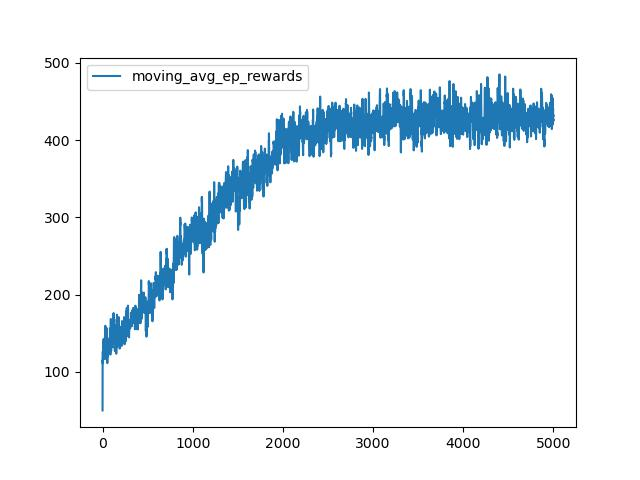
\includegraphics[width=.8\textwidth]{reward_plot.jpg}}
\caption{\label{figlabel2}The rewards for agents in 100,000 steps (every 20 records) }
\end{figure}

\item [2.]Loss: The training loss, measured as the Smooth L1 Loss between\cite{girshick2015fast}  \(TD_{e}\) and the \(TD_{t}\), increased over time. Periodic spikes in the loss were observed, corresponding to updates in the target network, but overall, the loss converged, indicating stable learning. The loss shows as following Fig.\ref{figlabel3}.

\begin{figure}[!t]
\centering
\subfigure{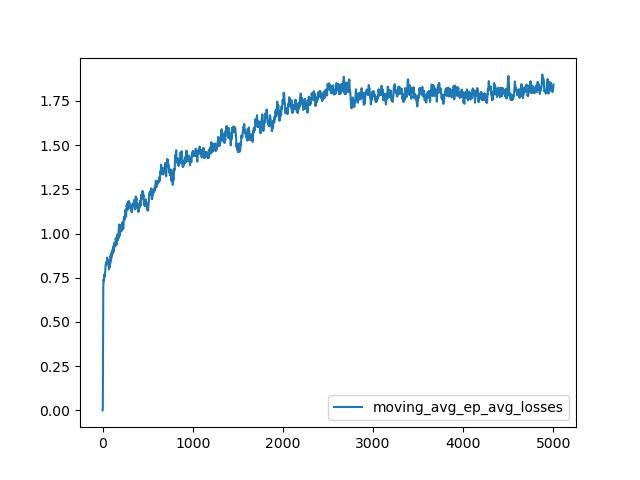
\includegraphics[width=.8\textwidth]{loss_plot.jpg}}
\caption{\label{figlabel3}The rewards for agents in 100,000 steps (every 20 records) }
\end{figure}

\item [3.]Stability: The agent's performance variance decreased over time, indicating stable and reliable gameplay.
\end{enumerate}

\subsection{Agent Performance}
The trained agent's performance was evaluated in several aspects. The game play efficiency of the agent was able to effectively shoot down aliens and avoid projectiles, demonstrating a good balance between offensive and defensive strategies. The agent's actions appeared smooth and well-coordinated, a result of learning from the sequential frames. Furthermore, strategy development of the agent developed specific strategies, such as focusing on eliminating columns of aliens to reduce the overall threat and timing shots to maximize hit probability. These strategies emerged naturally from the training process without explicit programming. The result of the agent show below Fig.\ref{figlabel4}

\begin{figure}[!t]
\centering
\subfigure{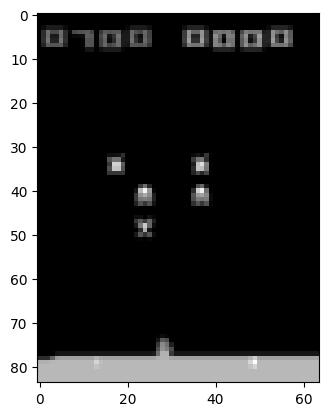
\includegraphics[width=.4\textwidth]{space_invaders3.png}}
\caption{\label{figlabel4}The result of the agent play the Space Invaders. }
\end{figure}

\section{Conclusion}

This project successfully applied Deep Reinforcement Learning (DRL) to the classic arcade game Space Invaders using the Double Deep Q-Network (DDQ) algorithm. Key findings include:

The Double Deep Q-Network (DDQ) algorithm enabled the agent to learn complex gameplay strategies from raw pixel data. The agent developed proficient offensive and defensive maneuvers.

Experience replay and target networks significantly stabilized the learning process. Experience replay broke the correlation between consecutive experiences, and the target network provided stable Q-value estimates, contributing to reliable learning outcomes.

The exploration decay policy ensured a balance between exploration and exploitation. This allowed the agent to explore the game environment sufficiently before refining its policy to maximize rewards.

The agent’s performance was quantitatively evaluated using metrics such as cumulative reward, loss, and stability. The agent consistently outperformed a random baseline and achieved scores, demonstrating the effectiveness of the DRL approach.

\newpage
\bibliographystyle{unsrt}
\bibliography{references}

% \newpage
\end{document}

